\documentclass[12pt,a4paper]{scrartcl}
    \usepackage[utf8]{inputenc}
    \usepackage{amsmath}
    \usepackage{amsfonts}
    \usepackage{amssymb}
    \usepackage{graphicx}

    \usepackage[bottom = 1in, left = 0.5in, right = 0.5in, top = 1in]{geometry}

    \usepackage[english]{babel}
    \usepackage[autostyle]{csquotes}
    \usepackage{mathptmx}

    \usepackage[labelfont=bf]{caption}

    \usepackage[default, scale=0.95]{opensans}

    \usepackage[T1]{fontenc}

    \usepackage{fixltx2e}

    % \addto\captionsenglish{\renewcommand{\figurename}{Supplementary Fig.}}
    % \addto\captionsenglish{\renewcommand{\tablename}{Supplementary Table}}

    \title{Figures}
    \date{}

    \begin{document}
\maketitle

\begin{figure}[h]
	\centering
	\includegraphics[scale = 1]{../../../graphs/fig1.pdf}
	\caption{Density plots showing the distribution of transmittance values measured by the ROV and the SUIT devices between 0-3 meters under sea ice. Numbers on top of the gray boxes identify the stations.}
\end{figure}

\clearpage
\newpage

\begin{figure}[h]
	\centering
	\includegraphics[scale = 1]{../../../graphs/fig1b.pdf}
	\caption{Boxplots, just an idea for the moment.}
\end{figure}

\begin{table}[ht]
    \centering
    \begin{tabular}{lrrrrr}
      \hline
     & Df & Sum Sq & Mean Sq & F value & Pr($>$F) \\ 
      \hline
    .\$source    & 1 & 3965.49 & 3965.49 & 2307.06 & 0.0000 \\ 
      Residuals   & 1720 & 2956.43 & 1.72 &  &  \\ 
       \hline
    \end{tabular}
    \end{table}

    \clearpage
    \newpage

\begin{figure}[h]
\centering
\includegraphics[scale = 1]{../../../graphs/fig2.pdf}
\caption{Violin plots of primary production calculated from ROV and SUIT transmittance data.}
\end{figure}

\clearpage
\newpage

\begin{figure}[h]
	\centering
	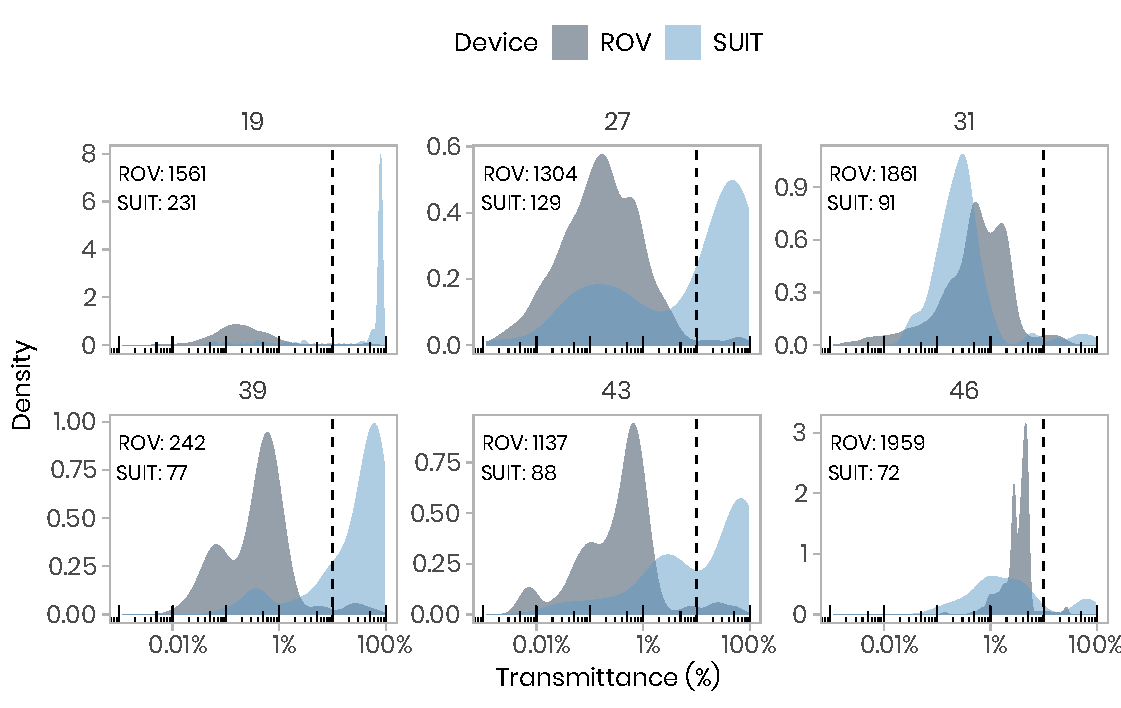
\includegraphics[scale = 1]{../../../graphs/fig3.pdf}
	\caption{Vertical profiles of daily primary production.}
\end{figure}

\clearpage
\newpage


\end{document}
